\documentclass[11pt,letterpaper]{article}
\usepackage[T1]{fontenc}
\usepackage[utf8]{inputenc}
\usepackage{lmodern}
\usepackage{amsmath,amssymb,amsthm,mathtools}
\usepackage[margin=1in,headheight=15pt]{geometry}
\usepackage{booktabs,longtable,array,enumitem}
\newcolumntype{P}[1]{>{\raggedright\arraybackslash}p{#1}}
\usepackage{xcolor,graphicx,tikz}
\usetikzlibrary{arrows.meta,positioning}
\usepackage{microtype,fancyhdr}
\usepackage[unicode,colorlinks=true,linkcolor=blue!45!black,urlcolor=blue!45!black,citecolor=blue!45!black]{hyperref}
\usepackage{bookmark}
\definecolor{ink}{HTML}{17334D}
\definecolor{accent}{HTML}{087E8B}
\definecolor{light}{HTML}{EDF4F7}
\setlength{\parskip}{0.42em}
\setlength{\parindent}{0pt}
\setlength{\emergencystretch}{2.5em}
\setlist{itemsep=0.25em,topsep=0.3em}
\pagestyle{fancy}
\fancyhf{}
\fancyhead[L]{\small\textcolor{ink}{GRH Lean: consequences and extensions}}
\fancyhead[R]{\small 25 November 2026}
\fancyfoot[C]{\thepage}
\renewcommand{\headrulewidth}{0.3pt}
\numberwithin{equation}{section}
\newtheorem{theorem}{Theorem}[section]
\newtheorem{proposition}[theorem]{Proposition}
\newtheorem{corollary}[theorem]{Corollary}
\newtheorem{lemma}[theorem]{Lemma}
\theoremstyle{definition}
\newtheorem{definition}[theorem]{Definition}
\theoremstyle{remark}
\newtheorem{remark}[theorem]{Remark}
\newcommand{\Q}{\mathbb{Q}}
\newcommand{\R}{\mathbb{R}}
\newcommand{\C}{\mathbb{C}}
\newcommand{\N}{\mathbb{N}}
\newcommand{\Z}{\mathbb{Z}}
\newcommand{\Cl}{\operatorname{Cl}}
\newcommand{\Gal}{\operatorname{Gal}}
\newcommand{\ord}{\operatorname{ord}}
\newcommand{\Nm}{\mathrm{N}}
\newcommand{\Rea}{\operatorname{Re}}
\newcommand{\Ima}{\operatorname{Im}}
\newcommand{\src}[1]{\href{https://github.com/lsernau/grh-lean/blob/72fead102f663d5c7a407964a13dc0cf9d977207/grh/src/#1}{\nolinkurl{#1}}}
\newcommand{\code}[1]{\nolinkurl{#1}}
\newcommand{\statusbox}[1]{\begin{center}\fcolorbox{accent}{light}{\begin{minipage}{0.92\linewidth}#1\end{minipage}}\end{center}}
\hypersetup{pdftitle={What can be transferred from grh-lean?},pdfauthor={Research analysis},pdfsubject={Source audit, mathematical consequences, and concrete routes beyond Dirichlet GRH}}
\begin{document}
\hypersetup{pageanchor=false}
\begin{titlepage}
\vspace*{0.8cm}
{\large\bfseries\color{accent} MATHEMATICAL RESEARCH REVIEW\par}
\vspace{1.0cm}
{\Huge\bfseries\color{ink} What can be transferred\\[0.15em] from \texttt{grh-lean}?\par}
\vspace{0.7cm}
{\Large A source audit, proved consequences,\\and a concrete route beyond Dirichlet GRH\par}
\vspace{1.0cm}
{\large Repository and mathematical transfer analysis\\25 November 2026 (Pacific time)\par}
\vspace{0.9cm}
\statusbox{\textbf{Finding.} The repository provides a substantial basis for further work. Its exported theorem covers Dirichlet \(L\)-functions over \(\Q\). Existing implications immediately reach abelian Dedekind zeta functions, Lindel\"of bounds, small quadratic nonresidues, and other classical targets. A genuine extension to a nonabelian field needs a new arithmetic estimate. This report isolates one such estimate explicitly.}
\vspace{0.5cm}
\textbf{Reviewed source}\\
\url{https://github.com/lsernau/grh-lean}\\
Commit \nolinkurl{72fead102f663d5c7a407964a13dc0cf9d977207}.

\textbf{Validation boundary}\\
Local source and hash audits were completed. Published independent checker logs for the exact snapshot were inspected and matched to their manifests. No full Lean build or kernel replay was run in this workspace. The added Lean interfaces are explicitly marked as uncompiled drafts.

\vfill
{\small The mathematical reductions proved here are explanatory or extracted consequences. No claim of a new proof of a further open conjecture, or of priority for an extracted lemma, is made.}
\end{titlepage}
\hypersetup{pageanchor=true}
\pagenumbering{roman}
\begingroup
\small
\setlength{\parskip}{0pt}
\tableofcontents
\endgroup
\newpage
\pagenumbering{arabic}
\section{Assessment and exact scope}\label{sec:assessment}

\subsection{Answer to the research question}

Yes: there are useful, rigorous transfers. They fall into three mathematically different categories.

\begin{enumerate}
\item \textbf{Consequences of the exported result.} Taking the repository's Dirichlet-GRH theorem as an established input, classical theorems whose only additional assumption is Dirichlet GRH can be applied. Examples include GRH for abelian extensions of \(\Q\), logarithmic bounds for the least quadratic nonresidue, and Lindel\"of bounds for Dirichlet \(L\)-functions. Their logical implication is established mathematics; it is not a new method invented in this review.
\item \textbf{Reusable proof infrastructure.} The general comparison of covolumes, indices, and heights, and the Landau transform argument, have interfaces that can be separated from the particular automorphic construction. Sections~\ref{sec:certificate} and \ref{sec:subset} give two precise extracted statements and their proofs.
\item \textbf{New research beyond the theorem's scope.} The most concrete target identified here is the \(L\)-function of a nontrivial ideal-class character of \(\Q(\sqrt{-23})\). Its RH would imply RH for the cubic field generated by a root of \(X^3-X-1\). Section~\ref{sec:principal-target} reduces this target to a specific one-sided inequality for principal prime-power ideals. The required arithmetic inequality is not proved here.
\end{enumerate}

The distinction matters. A formal proof of a statement about one class of functions does not, by virtue of using sophisticated mathematics internally, prove the analogous assertion for every class of functions appearing in its proof. Conversely, the absence of a short human exposition does not negate a successful proof-kernel verification. The assessment below respects both points.

\subsection{The fixed source snapshot}

This review uses commit
\[
\text{\small\nolinkurl{72fead102f663d5c7a407964a13dc0cf9d977207}}
\]
of \code{lsernau/grh-lean}. Both editions pin Lean \(4.35.0\) and Mathlib commit
\[
\text{\small\nolinkurl{56a005855ea17e0b0958f73ec801ae140b0a1679}}.
\]
The readable edition is the main source for mathematical interpretation; the compact edition is the practical first choice for an independent rebuild. The repository credits Levent Alp\"oge and Claude for the proof, and describes the shortening as a collaboration involving Luke Sernau, colleagues at Anthropic, and Claude \cite{repo,announcement}.

The local audit found the following exact source counts. \emph{Code lines} means nonblank lines remaining after masking comments and strings; it is a lexical measure, not a measure of mathematical complexity.

\begin{center}
\begin{tabular}{lrr}
\toprule
Measure & Readable & Compact\\
\midrule
Lean files under \code{src} &803&794\\
Files under \code{Lib} &495&573\\
Files under \code{New} &306&219\\
Total source lines &477,124&112,827\\
Nonblank lines, including comments &432,527&95,030\\
Approximate nonblank code lines &299,902&76,149\\
Local modules imported transitively by \code{Main} &803&794\\
\bottomrule
\end{tabular}
\end{center}

Every source module belongs to the module-import closure of \code{Main}. This does not imply that every declaration in those modules occurs in the proof term of a final theorem. No import cycle was found, and no \code{Lib} module imports a \code{New} module. The inventories and the script that produced them are included in the archive.

\subsection{What the five theorems say}

The decisive interface is \src{Statements.lean}, which imports only Mathlib, together with \src{Main.lean}. It is useful to state the content in conventional mathematical notation.

\begin{longtable}{P{0.39\linewidth}P{0.55\linewidth}}
\toprule
Public declaration & Content\\
\midrule
\endhead
\code{riemannHypothesis} & Mathlib's ordinary RH for \(\zeta\).\\
\code{riemannZeta_eq_zero_re} & A zero of \(\zeta(s)\), excluding negative even integers and the separately excluded pole point \(1\), has real part \(1/2\).\\
\code{LFunction_ne_zero_of_half_lt_re} & For every nonzero modulus and every Dirichlet character \(\chi\), \(L(s,\chi)\ne0\) if \(\Rea s>1/2\), except for the principal-character pole at \(s=1\).\\
\code{LFunction_eq_zero_re} & For every such \(\chi\), a zero in \(0<\Rea s<1\) has real part \(1/2\).\\
\code{LFunction_eq_zero_re_of_isPrimitive} & The preceding statement restricted to primitive characters.\\
\bottomrule
\end{longtable}

There is no hidden primitive-character restriction in the stronger two Dirichlet statements. In particular, the result covers characters induced from a smaller conductor. Their additional Euler factors can have zeros on \(\Rea s=0\), so the open-strip formulation is the appropriate one.

The pole exclusions are also substantive. Lean represents functions by total maps, so a meromorphic function's conventional value at a pole must be excluded when expressing zero location. Excluding \(s=1\) for a principal character is correct, and does not leave a gap at an ordinary point of its analytic domain.

The exact official Mathlib definitions at the pinned commit were separately retrieved. The zeta function and Dirichlet \(L\)-function are the existing analytic continuations, agreeing with their Dirichlet series in \(\Rea s>1\); they are not newly invented functions named after those objects. This checks the outer statement boundary. It is not a reproof of all of Mathlib.

\subsection{Validation evidence and its limits}

The primary independent verification page by Andrew Sutherland is stamped 26 November 2026, 02:50 UTC, which is 25 November in Pacific time. It reports that both editions completed paranoid Comparator checking, with statement comparison, the axiom audit, Lean kernel checks, and the supplied external checkers. A second compact run also passed. A smaller-machine readable run was stopped for memory use; its lack of a verdict is separate from the successful larger-machine run \cite{checks}.

This review retrieved the relevant logs and checked source identity locally:

\begin{itemize}
\item All 1,625 entries in the verifier's source-file checksum manifest match the checkout. The only tracked files outside that list are the repository-root license and README.
\item The SHA-256 of the local Git archive matches the verifier's reported archive hash:
\begin{center}\small
\nolinkurl{9138cf2f5862e64f823ed676e8d37333c0717e1a13cd8f74f6b735ab2d1ba57c}.
\end{center}
\item All 23 selected downloaded evidence files covered by the verifier's checksum list match that list.
\end{itemize}

These matches substantiate that the source examined here is the source named in the successful verification evidence. The checksums and logs share a provenance; checking them is not the same operation as rerunning the proof kernels.

The local lexical audit found no proof placeholders or custom axioms in either \code{src} tree, and no occurrences of the execution or elaboration mechanisms included in the audit's watch list. Each top-level \code{Challenge.lean} does contain five \code{sorry} placeholders. They are comparison targets, outside the source import closure and default build targets; treating them as gaps in \code{Main} would be an error. The downloaded axiom outputs name only \code{propext}, \code{Classical.choice}, and \code{Quot.sound}.

\statusbox{\textbf{Local verification status.} Source inspection, module inventory, exact hash matching, and the arithmetic experiments in this archive were executed. Lean, Lake, and independent proof checkers were not installed in this workspace, so no local compilation or proof replay is claimed. The additional Lean interfaces have not inherited the upstream verification status.}

The repository can therefore be treated as a substantial formally checked artifact for its actual statements, supported by published independent evidence. Understanding how its construction behaves under a change of arithmetic setting remains a separate mathematical task.

\section{The mathematical mechanism}\label{sec:mechanism}

\subsection{The error term actually controlled}

Fix a positive modulus \(q\), and a suitable prime \(d\equiv7\pmod8\) coprime to \(q\). Write
\(\chi_d(n)=(n/d)\) for the quadratic character. The principal statistic is
\begin{equation}\label{eq:R}
R_{d,q}(x)=
\sum_{\substack{n\le x\\n\equiv1\;(\mathrm{mod}\ q)}}
\Lambda(n)(1-\chi_d(n))
\left(\frac1n-\frac1x\right)
-\frac{\log x}{\varphi(q)}-c_{d,q}.
\end{equation}
Here \(\Lambda(p^r)=\log p\), and \(\Lambda(n)=0\) otherwise; \(c_{d,q}\) is the normalizing constant for which the remainder tends to zero. The prime sum has nonnegative terms. Its weights select a quadratic splitting condition and a rational congruence condition. The smoothing factor makes the transform and its zero residues particularly manageable.

The endpoint of the arithmetic argument is an \emph{upper} bound:
\begin{equation}\label{eq:one-sided}
R_{d,q}(x)\le x^{-1/2+\varepsilon}
\quad\text{for all sufficiently large \(x\), for each \(\varepsilon>0\).}
\end{equation}
It is not first proved as an absolute-value estimate. The passage from this one-sided statement to a zero-free half-plane is an essential part of the proof.

For the arithmetic construction, \(q_0\) is a multiple of \(18480\), and \(d\) lies in a specified class modulo \(q_0\). This restriction is internal: the final theorem raises an arbitrary modulus to a suitable multiple and then uses change-of-level identities. It does not restrict the final GRH statement to a subset of moduli.

\subsection{Three estimates for a common object}

The source constructs finite-dimensional spaces of automorphic forms and maps formed from chains of theta lifts. Its auxiliary field is of the special form
\[
E=\Q(\sqrt{-d},\zeta_{q_1}).
\]
This is a CM field, abelian over \(\Q\). The proof uses both its archimedean embeddings and arithmetic at finite primes. Replacing this field by a general extension is not a change of notation.

The structure of the comparison can be stated without reproducing the entire construction. Let \(D_{\rm tar}\) be the target dimension, and \(n\) the size of a linearly independent family selected from images of integral source forms. The two quantitative invariants are:

\begin{itemize}
\item \(V\), an upper bound on the logarithm of a Gram determinant, or squared covolume, of the lifted family;
\item \(\delta\), a logarithmic index bound measuring the loss needed to make the family integral at all relevant finite places.
\end{itemize}

Three substantial inputs control these invariants.

\begin{enumerate}
\item \textbf{Short forms.} There are enough integral source vectors with small archimedean norms, and their images have controlled denominators.
\item \textbf{Almost spanning.} A controlled number of translates of the images span a subspace of dimension at least
\[
\left(1-\frac4{b^2}\right)D_{\rm tar}.
\]
\item \textbf{Long integral forms.} A product-formula and determinant-height argument gives a lower bound for \(V+2\delta\). This uses twists chosen separately at finite primes, and a quantitative comparison between twisted and untwisted determinants.
\end{enumerate}

The relevant source interfaces are \src{New/Reduction/ShortAndEnough.lean},
\src{New/Determinant/Twist/LongForms.lean}, and
\src{New/Reduction/Lattices/TwistedLattice.lean}. The full arithmetic construction proves the hypotheses of these interfaces; none should be assumed automatically in a new setting.

\subsection{Cancellation of the main amount}

Suppressing error terms for a moment, the two bounds have the shape
\begin{equation}\label{eq:schematic}
\mathcal M\ \le\ \frac{V+2\delta}{D_{\rm tar}}\
\le\ \mathcal M-\frac{n}{D_{\rm tar}}m\,\mathcal R.
\end{equation}
The same main amount \(\mathcal M\) occurs on both sides. Its cancellation leaves a bound on the desired remainder \(\mathcal R\), amplified by the number \(m\) of lifts.

The implemented theorem \code{New.star_inequality} is
\begin{equation}\label{eq:star}
m\,\mathcal R\le fa(\log b)^5,
\end{equation}
where \(f\) is the number of infinite places of the auxiliary field and \(a=xb\). It is proved in \src{New/Reduction/MainInequality.lean}. This short comparison is supported by the much larger preceding construction.

\begin{figure}[ht]
\centering
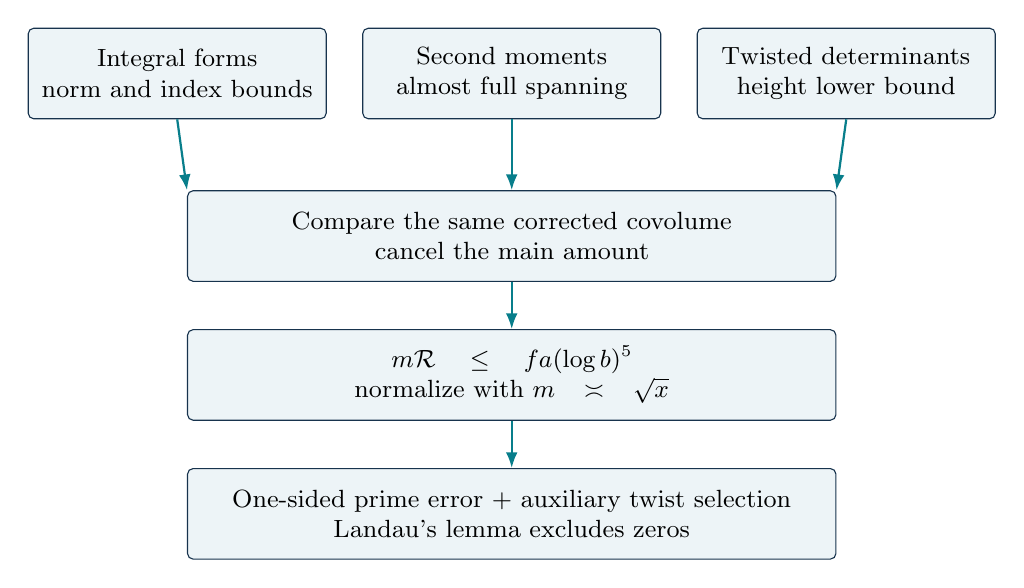
\begin{tikzpicture}[
  box/.style={draw=ink,rounded corners=2pt,fill=light,align=center,text width=3.55cm,minimum height=1.15cm,font=\small},
  wide/.style={box,text width=8.0cm},
  arr/.style={-{Latex[length=2mm]},thick,draw=accent}
]
\node[box] (short) {Integral forms\\norm and index bounds};
\node[box,right=0.45cm of short] (span) {Second moments\\almost full spanning};
\node[box,right=0.45cm of span] (long) {Twisted determinants\\height lower bound};
\node[wide,below=0.9cm of span] (compare) {Compare the same corrected covolume\\cancel the main amount};
\node[wide,below=0.6cm of compare] (prime) {\(m\mathcal R\le fa(\log b)^5\)\\normalize with \(m\asymp\sqrt{x}\)};
\node[wide,below=0.6cm of prime] (analytic) {One-sided prime error + auxiliary twist selection\\Landau's lemma excludes zeros};
\draw[arr] (short.south) -- (compare.north west);
\draw[arr] (span.south) -- (compare.north);
\draw[arr] (long.south) -- (compare.north east);
\draw[arr] (compare) -- (prime);
\draw[arr] (prime) -- (analytic);
\end{tikzpicture}
\caption{The reusable logical structure. Each upper box represents a large theorem with arithmetic hypotheses, not an available black box for every \(L\)-function.}
\end{figure}

The constants also have to match accurately. The source identifies cancellations involving period normalizations, the expected value of the weighted prime sum, the archimedean sizes of the lifts, and the level. Matching only leading orders would not suffice if a residual main term exceeded the final error.

\subsection{Why the square root appears}

The normalization of \eqref{eq:star} gives the source inequality
\begin{align}\label{eq:normalized}
R_{d,q_0}(x)\le {}&
\frac{\varphi(q_0)(\log b)^6}{m}
+|R_{d,q_0}(x_1)|\\
&+(\log b)|R_{d,1}(x_1)|.\nonumber
\end{align}
The parameters are arranged so that
\[
\sqrt{x}\le m\le2\sqrt{x},
\qquad
\log b\le2x^\varepsilon,
\qquad
\log x_1\ge x^{\varepsilon/12}.
\]
The two terms at \(x_1\) are controlled by ordinary prime-number-theorem estimates for fixed characters. At that enormous scale they are smaller than the required power of \(x\). No GRH input is used to prove those large-scale error bounds.

At integer \(x\), the source obtains, for \(0<\varepsilon<1/100\),
\[
R_{d,q_0}(x)\le
(64\varphi(q_0)+3)x^{-1/2+6\varepsilon}.
\]
Changing the small parameter, absorbing constants, and comparing a real \(x\) with its integer part gives \eqref{eq:one-sided}. These steps are explicit in \src{New/Reduction/OneSidedBound.lean}.

This is a scale argument rather than a practical numerical algorithm. The enormous auxiliary weights, levels, and dimensions are compatible with an asymptotic theorem, but the construction is not presented as a competitive method for computing prime counts.

\subsection{How a one-sided bound excludes zeros}

Put \(E(v)=R_{d,q}(e^v)\). Its transform
\[
\mathcal T(s)=\int_0^\infty E(v)e^{(1-s)v}\,dv
\]
has a meromorphic continuation in \(\Rea s>0\). Write \(L^\circ(s,\chi)\) for the entire version of a Dirichlet \(L\)-function, with its principal pole removed. Away from the separately treated points, its residue is
\begin{equation}\label{eq:residue}
\operatorname*{Res}_{s=\rho}\mathcal T(s)
=
\frac{
\sum_{\chi\bmod q}\ord_\rho L^\circ(s,\chi)
-
\sum_{\chi\bmod q}\ord_\rho L^\circ(s,\chi\chi_d)}
{\varphi(q)\rho(1-\rho)}.
\end{equation}

One cannot simply declare the numerator positive: it is a difference. If an untwisted and a twisted function vanish at the same point, cancellation is possible.

For a hypothetical zero \(\rho\) with \(\Rea\rho>\beta>1/2\), the source first chooses \(d\) such that every twisted function is zero-free in
\[
\Rea s\ge\beta,\qquad |\Ima s|\le|\Ima\rho|.
\]
A zero-density estimate for quadratic twists provides this choice. For that \(d\), the second sum in \eqref{eq:residue} vanishes throughout the relevant box. The remaining multiplicities are nonnegative integers. At real \(s\in(\beta,1)\) the denominator \(s(1-s)\) is positive, and above \(1\) the entire factors have no zeros.

The abstract lemma \code{New.IsPolar.landau}, in \src{Lib/Analytic/Landau.lean}, says that an eventual upper bound
\[
E(v)\le e^{(\beta-1)v}
\]
and nonnegative real residues rule out every pole with real part greater than \(\beta\). One way to see the mechanism is to consider
\[
K e^{\beta v}-E(v)e^v\ge0
\]
with a large enough constant \(K\), and apply Landau's theorem to the Laplace transform of this positive density. A positive measure cannot have an analytic Laplace transform through its finite real abscissa of convergence; the sign of a possible real pole yields the contradiction.

Consequently the residue at the proposed \(\rho\) is zero. Its numerator is a sum of nonnegative integers containing the multiplicity of the proposed zero, which is impossible. This gives nonvanishing on the right; the functional equation gives the critical-line statement.

The transfer lesson is precise. If the new statistic has \emph{mixed} zero multiplicities as in \eqref{eq:residue}, a noncancellation mechanism is required. If it is built instead from a full product with only positive multiplicities, that auxiliary analytic step may disappear. The cubic-field reduction in Section~\ref{sec:principal-target} exploits the second possibility.

\section{Two extracted transfer results}\label{sec:lemmas}

The following statements make two reusable parts of the proof explicit. They are proved here as mathematical deductions. Neither is claimed to be new in the literature, and neither constitutes a new resolution of a conjecture.

\subsection{A quantitative comparison certificate}\label{sec:certificate}

\begin{proposition}[Covolume comparison with explicit losses]\label{prop:certificate}
Let \(D>0\), \(m>0\), \(0<\alpha\le1\), and \(\alpha D\le n\le D\). Let \(M,U,L,I\ge0\), and let \(R,V,\delta\) be real numbers satisfying
\begin{equation}\label{eq:certificate-inputs}
D(M-L)\le V+2\delta,\qquad
V\le n(M-mR+U),\qquad
\delta\le DI.
\end{equation}
Then
\begin{equation}\label{eq:certificate-sharp}
nmR\le nU+D(L+2I)-(D-n)M,
\end{equation}
and in particular
\begin{equation}\label{eq:certificate}
R\le\frac{U}{m}+\frac{L+2I}{\alpha m}
\le\frac{U+L+2I}{\alpha m}.
\end{equation}
\end{proposition}

\begin{proof}
Combining the three hypotheses gives
\[
D(M-L)\le n(M-mR+U)+2DI.
\]
Rearrangement is exactly \eqref{eq:certificate-sharp}. Because \(D-n\ge0\) and \(M\ge0\), dropping the last term increases the right side. Divide by \(nm>0\), and use \(D/n\le1/\alpha\) together with \(L+2I\ge0\). The last inequality follows from \(U\ge0\) and \(\alpha\le1\).
\end{proof}

Here \(U\) is the loss in the upper norm estimate, \(L\) the loss in the lower estimate, and \(I\) the loss from denominators. This formulation identifies what a proposed adaptation must actually prove. Having a family of theta lifts is insufficient; its three normalized losses and its surviving rank must satisfy a quantitative certificate.

If, after all normalizations, the combined loss \(U+(L+2I)/\alpha\) is \(O_\eta(x^\eta)\) and \(m\ge x^\theta\), one obtains an upper bound of order \(x^{-\theta+\eta}\). This definition includes any loss from a varying spanning fraction \(\alpha\). With the particular Dirichlet quadratic-twist criterion from this repository, this excludes zeros only strictly to the right of
\[
\max\left\{\frac12,\,1-\theta+\eta\right\}.
\]
The \(1/2\) floor here belongs to that twist-selection theorem. No conclusion beyond its domain can be obtained just by increasing \(m\).

\subsection{Why the certificate is expensive to satisfy}

The apparently weak condition \(n\ge D/2\) is enough for the final division. It is not enough for the arithmetic lower bound that precedes it.

In \src{New/Determinant/Twist/LongForms.lean}, a missing basis vector has a completion cost bounded by
\[
2x_1^2b^2+b.
\]
The source supplies \(D-n\le4D/b^2\), yielding total cost at most
\[
4D(2x_1^2+b^{-1})\le Db
\]
under the chosen scale inequalities. A fixed positive missing fraction would instead leave a term of order \(Dx_1^2b^2\). Almost full spanning is therefore a mathematical necessity of this lower-bound argument, even though the last line of the proof uses only a positive fraction of the dimension.

The denominator comparison is equally informative. The allotted budget in \src{New/Determinant/Twist/FitTwists.lean} is
\[
\frac{fa(\log b)^3}{mk},
\qquad a=xb.
\]
The explicit local-defect estimate in \src{New/Congruences/FitTwistsExist.lean} has size
\[
O\!\left(f\frac{m}{k}b\log b\right).
\]
Their quotient has the form
\begin{equation}\label{eq:budget-ratio}
O\!\left(\frac{m^2}{x(\log b)^2}\right).
\end{equation}
Thus \(m\asymp\sqrt{x}\) leaves logarithmic room. Taking a larger power of \(x\) while keeping the subpower scale choices would require better loss estimates. More generally, if a normalized loss grows like \(m\), division by \(m\) leaves a constant error and the desired decay disappears.

\subsection{Only sufficiently many auxiliary primes are needed}\label{sec:subset}

The published criterion asks for the arithmetic bound at every permitted auxiliary prime. Its proof actually requires only one prime that is simultaneously arithmetically successful and analytically good for each possible zero.

\begin{theorem}[A large successful set suffices]\label{thm:subset}
Let \(q\) be a positive multiple of \(8\), let \(a\) be coprime to \(q\) with \(a\equiv7\pmod8\), and fix \(1/2<\beta<1\). Let \(S\) be a set of primes \(d\equiv a\pmod q\). Suppose:
\begin{enumerate}
\item For every \(d\in S\), \(R_{d,q}(x)\le x^{\beta-1}\) for all sufficiently large real \(x\). The threshold may depend on \(d\).
\item If \(A_S(X)=\#\{d\in S:d\le X\}\) and \(c=(\beta-1/2)/18\), then
\[
\frac{A_S(X)}{X^{1-c}}
\quad\text{is unbounded for positive integer \(X\).}
\]
\end{enumerate}
Then \(L(\rho,\chi)\ne0\) for every character modulo \(q\) and every \(\rho\ne1\) with \(\Rea\rho>\beta\).
\end{theorem}

\begin{proof}
Fix a proposed \(\rho\) and put \(T=|\Ima\rho|\) and \(\delta=(\beta-1/2)/9\). The theorem
\code{zero_density_quadTwist} in \src{Lib/Analytic/QuadraticTwist.lean} bounds by
\[
O_{q,\beta,T}\!\left(X^{1-\delta/2}\right)
=O_{q,\beta,T}(X^{1-c})
\]
the number of permitted primes \(d\le X\) for which some quadratic twist of a character modulo \(q\) has a zero in
\(\Rea s\ge\beta,\ |\Ima s|\le T\).

By the second hypothesis, \(S\) cannot be contained in this exceptional set. Choose \(d\in S\) outside it. For this fixed \(d\), the first hypothesis provides the required eventual one-sided bound. All the twisted multiplicities in \eqref{eq:residue} vanish in the chosen box. The remaining real residues are nonnegative; Landau's lemma therefore makes the residue at \(\rho\) zero. The denominator is nonzero and the numerator is a sum of nonnegative integers. In particular the multiplicity of a zero of the proposed \(L(s,\chi)\) must be zero, a contradiction.
\end{proof}

The order of quantifiers is essential: first choose \(\rho\), then a successful \(d\), then use the eventual estimate for that \(d\). No uniform bound on the thresholds \(X_d\) is required.

\begin{corollary}\label{cor:density}
Each of the following conditions on \(S\) is sufficient for the second hypothesis:
\begin{enumerate}
\item positive upper relative density among the primes in the permitted residue class;
\item \(\limsup_{X\to\infty}\log(1+A_S(X))/\log X=1\);
\item divergence of \(\sum_{d\in S}(\log d)/d\).
\end{enumerate}
\end{corollary}

\begin{proof}
For the first, the prime number theorem for a fixed progression gives counts on a sequence of order \(X/\log X\), and \(X^c/\log X\to\infty\). For the second, a bound \(A_S(X)=O(X^{1-c})\) contradicts the displayed upper exponent. For the third, such a counting bound would make the sum converge by partial summation, since the resulting tail integral is bounded by a constant times
\(\int_2^\infty (\log t)t^{-1-c}\,dt\).
\end{proof}

To recover GRH, use the theorem for every \(\beta\in(1/2,1)\); the successful set may depend on \(\beta\). A single set with counting exponent \(1\), on which the bound holds for every positive \(\varepsilon\) in the form \eqref{eq:one-sided}, also suffices.

This weakening could be useful when a new arithmetic construction works only for many auxiliary parameters rather than all of them. It is a reduction of required hypotheses, not a construction of those parameters or a new zero-free region by itself.

\section{Other questions reached by the exported theorems}\label{sec:consequences}

Throughout this section the repository's exported RH and Dirichlet-GRH theorems are used as inputs. This is a mathematical dependency, not an assertion that the present workspace performed their kernel verification. The classical implications listed below are not new theorems of this report.

\subsection{Every abelian Dedekind zeta function over \texorpdfstring{\(\Q\)}{Q}}

\begin{proposition}[Finite products preserve critical-line zero location]\label{prop:product}
Let \(F_1,\ldots,F_r\) be holomorphic in \(0<\Rea s<1\), and suppose each has all its zeros in that strip on \(\Rea s=1/2\). Then the same is true of \(\prod_jF_j\).
\end{proposition}

\begin{proof}
At any point in the strip, a finite product of nonzero complex numbers is nonzero. A zero of the product therefore belongs to at least one factor, whose hypothesis gives the conclusion.
\end{proof}

\begin{corollary}[Abelian Dedekind GRH]\label{cor:abelian}
For every finite abelian extension \(A/\Q\), every zero of \(\zeta_A(s)\) in \(0<\Rea s<1\) lies on \(\Rea s=1/2\).
\end{corollary}

\begin{proof}
Kronecker--Weber places \(A\) in a cyclotomic field. Associate to each character of \(\Gal(A/\Q)\) its primitive Dirichlet character, and let \(X_A\) be this finite set. The exact factorization is
\begin{equation}\label{eq:abelian}
\zeta_A(s)=\prod_{\chi\in X_A}L(s,\chi).
\end{equation}
This equality holds meromorphically; it follows from the Euler factors in the convergence half-plane and continuation. Every factor is holomorphic in the open strip, because its only possible pole is at \(1\). Apply the repository's Dirichlet-GRH theorem and Proposition~\ref{prop:product}.
\end{proof}

The standard factorization and Kronecker--Weber theorem are explicitly stated in Sutherland's course notes \cite{kronecker}. This corollary includes quadratic and cyclotomic fields and their subfields. The primitive-character convention matters for exact equality: writing all factors at one larger imprimitive modulus can remove finite Euler factors. Those factors do not vanish in the open strip, but using the primitive factors avoids the extra correction.

This is a realistic first formalization project. Its new work is the formal factorization interface, not a new estimate for zeros. The included Lean file proves only the generic product and Dirichlet-product parts; it does not pretend that \eqref{eq:abelian} has been formalized there.

\subsection{Real zeros and central signs}

\begin{proposition}[Real nonprincipal characters]\label{prop:positive}
Let \(\chi\) be a real-valued, nonprincipal Dirichlet character. Then
\[
L(\sigma,\chi)>0\quad(\sigma>1/2),
\qquad
L(1/2,\chi)\ge0.
\]
\end{proposition}

\begin{proof}
For real \(\sigma>1\), the absolutely convergent Euler product has positive factors, so \(L(\sigma,\chi)>0\). Because \(\chi\) is real, analytic continuation is real-valued on the real axis. Because it is nonprincipal, it is entire. The exported half-plane theorem says it is nonzero on the connected real interval \((1/2,\infty)\). A continuous real-valued function cannot change sign there without vanishing. It is therefore positive throughout that interval, and continuity at \(1/2\) gives the nonnegative endpoint value.
\end{proof}

This removes real zeros in \((1/2,1)\), including the possible exceptional zeros near \(1\). It does not prove strict positivity at \(1/2\). The nonprincipal assumption is essential: a principal function has a pole at \(1\), so the connectedness argument across that point is unavailable. Likewise, zero location does not assert simplicity or any bound on multiplicities.

\subsection{Quantitative and elementary consequences}

The following are representative established implications with hypotheses matching the exported result. Logarithms are natural. Constants in \(O_\varepsilon\) may depend on \(\varepsilon\).

\begin{longtable}{P{0.24\linewidth}P{0.48\linewidth}P{0.20\linewidth}}
\toprule
Question & Consequence after importing the result & Source / dependency\\
\midrule
\endhead
Least quadratic nonresidue & For prime \(p\ge5\), the least positive nonresidue is \(<(\log p)^2\). & Dirichlet GRH; \cite{lls}, Cor.~1.1.\\[0.3em]
Least prime in a progression & If \(q>3\), \((a,q)=1\), then \(P(a,q)\le(\varphi(q)\log q)^2\). & Dirichlet GRH; \cite{lls}, Cor.~1.2.\\[0.3em]
Lindel\"of bounds & For primitive \(\chi\) of conductor \(q\), \(\lvert L(1/2+it,\chi)\rvert\ll_\varepsilon(q(2+|t|))^\varepsilon\). & Dirichlet GRH and standard analytic estimates; \cite{chandee}.\\[0.3em]
M\"obius cancellation & \(\sum_{n\le x}\mu(n)=O_\varepsilon(x^{1/2+\varepsilon})\) for every \(\varepsilon>0\). & Ordinary RH; \cite{sound}.\\[0.3em]
Primes in short intervals & For every \(x\ge2\), a prime lies in \((x-\frac4\pi\sqrt{x}\log x,x]\). & Ordinary RH; \cite{dudek}, Thm.~2.\\[0.3em]
Divisor-sum inequality & For \(n\ge1\), \(\sum_{d\mid n}d\le H_n+e^{H_n}\log H_n\), with equality only at \(n=1\). & Equivalent to RH; \cite{lagarias}, Thm.~1.1.\\
\bottomrule
\end{longtable}

The least-nonresidue and least-prime statements use the corrected arXiv version of Lamzouri--Li--Soundararajan \cite{lls}. The explicit constants here are useful examples, not assertions of the current optimal bounds. The divisor inequality is an elementary reformulation of the same RH difficulty, rather than an independent analytic breakthrough.

For M\"obius cancellation, the exponent must retain \(\varepsilon>0\). One must not replace it by the much stronger unit-constant bound \(|\sum_{n\le x}\mu(n)|<\sqrt{x}\). The transfer concerns the stated asymptotic estimate. Similarly, Lindel\"of for this family does not imply a corresponding theorem for every higher-degree automorphic \(L\)-function.

These consequences can be used rigorously in ordinary mathematical proofs once their cited implication theorems are supplied. A Lean development needs those bridges as actual formal theorems; calling the result in \code{Main} does not automatically add all of classical analytic number theory to the library.

\subsection{Why several prominent conjectures are not reached}

\paragraph{Artin's primitive-root conjecture.}
The usual conditional proof needs effective splitting estimates in Kummer fields
\[
\Q(\zeta_k,a^{1/k}),\qquad k\text{ squarefree}.
\]
These are generally nonabelian over \(\Q\). For example, the splitting field of \(X^3-2\) is \(\Q(\zeta_3,\sqrt[3]2)\). The cubic is irreducible by Eisenstein's criterion, and its discriminant \(-108\) is not a square, so the Galois group is \(S_3\). Its zeta factorization involves a two-dimensional Artin representation in addition to one-dimensional factors.

Dirichlet GRH controls the latter; it does not supply the missing degree-two zero estimate. Lenstra's formulation makes the needed Dedekind-zeta hypotheses explicit \cite{lenstra}. Thus the familiar assertion that Artin follows from GRH cannot be used here without specifying the larger family of \(L\)-functions.

\paragraph{Legendre's conjecture.}
The displayed short-interval theorem does not place a prime between every pair of consecutive squares. At \(x=(n+1)^2\), its guaranteed interval has length
\[
\frac4\pi(n+1)\log((n+1)^2).
\]
Dividing by the available gap \(2n+1\) gives a ratio asymptotic to \((4/\pi)\log n\), which diverges. The interval extends too far below \(n^2\). This is a precise failure of that deduction, not a proof that RH logically cannot imply Legendre by some other argument.

\paragraph{Twin primes, binary Goldbach, and correlations.}
The repository locates zeros and controls certain one-variable prime sums. It supplies no argument for the shifted prime correlations required for twin primes or the additive correlations required for binary Goldbach. An analogous warning applies to inferring all M\"obius correlations from a bound for \(\sum_{n\le x}\mu(n)\). No solution of those problems is established by this analysis.

\paragraph{Central nonvanishing, simplicity, and BSD.}
An \(L\)-function may have a zero exactly on the critical line with any multiplicity without contradicting GRH. In particular, statements about values or derivatives at the central point require additional information. The occurrence of Galois representations and Selmer groups as tools inside the repository is not a proof of the Birch--Swinnerton-Dyer conjecture or a general special-value formula.

\section{A concrete target beyond Dirichlet GRH}\label{sec:cubic}

\subsection{The field and the missing factor}

Let
\[
F=\Q(\theta),\qquad \theta^3-\theta-1=0,
\qquad K=\Q(\sqrt{-23}),
\]
and let \(H\) be the splitting field of the cubic. The following identities are classical; the example and its factorization are described in Venkatesh's lectures, in notes by Feng \cite{venkatesh}, and the Hilbert-class-field identification also occurs in Schoof's paper \cite{schoof}.

\begin{proposition}\label{prop:cubic}
The group \(\Cl(K)\) is cyclic of order \(3\), and \(H\) is its Hilbert class field. If \(\psi\) is either nontrivial character of \(\Cl(K)\), then
\begin{align}
\zeta_F(s)&=\zeta(s)L_K(s,\psi),\label{eq:cubic}\\
\zeta_H(s)&=\zeta_K(s)L_K(s,\psi)^2
=\zeta(s)L(s,\chi_{-23})L_K(s,\psi)^2.\label{eq:galois}
\end{align}
\end{proposition}

\begin{proof}
The only possible rational roots of \(X^3-X-1\) are \(\pm1\), and neither is a root. Its discriminant is
\[
-4(-1)^3-27(-1)^2=-23.
\]
It is squarefree, so the order \(\Z[\theta]\) is maximal; it is nonsquare, so the transitive Galois group is \(S_3\), with quadratic subfield \(K\).

Reduced positive definite primitive forms of discriminant \(-23\) have first coefficient at most \(\sqrt{23/3}<3\). Enumerating the possibilities gives exactly
\[
(1,1,6),\qquad (2,1,3),\qquad (2,-1,3).
\]
The classical ideal-class/form correspondence therefore gives \(h_K=3\).

The extension \(H/K\) is cyclic of degree \(3\). No prime other than \(23\) ramifies. Modulo \(23\),
\[
X^3-X-1=(X-10)^2(X-3).
\]
The simple root lifts over \(\Q_{23}\), so the local decomposition group fixes a root and is contained in an order-two stabilizer. The quadratic field is ramified at \(23\), so inertia is exactly that order-two subgroup; its intersection with \(A_3=\Gal(H/K)\) is trivial. Thus \(H/K\) is unramified at finite places. There are no real places of \(K\) to consider. Its degree is the class number, so class field theory identifies it with the Hilbert class field.

Let \(V\) be the standard two-dimensional representation of \(S_3\). The permutation representation on three roots is \(\mathbf1\oplus V\); hence its Artin \(L\)-function gives \(\zeta_F=\zeta L_\Q(V)\). Inducing either nontrivial character of \(A_3\) gives \(V\): the resulting character takes values \(2,0,-1\) on the identity, transpositions, and three-cycles. Compatibility of Artin \(L\)-functions with induction identifies \(L_\Q(V)\) with \(L_K(\psi)\). The two nontrivial characters induce isomorphic representations and give the same \(L\)-function. Finally the regular representation of \(S_3\) is \(\mathbf1\oplus\mathrm{sgn}\oplus V^{\oplus2}\), proving \eqref{eq:galois}.
\end{proof}

The missing factor \(L_K(s,\psi)\) is a Hecke \(L\)-function over a quadratic field, of degree two when viewed over \(\Q\). Its analytic continuation is known; the new issue is its critical-strip zeros. Under the repository's results for \(\zeta\) and \(L(s,\chi_{-23})\), RH for \(L_K(s,\psi)\), RH for \(\zeta_F\), and RH for \(\zeta_H\) are equivalent. Inside the strip all factors in \eqref{eq:cubic}--\eqref{eq:galois} are holomorphic, so zeros cannot be canceled by poles.

This is a better first extension target than another quadratic field, whose zeta function is already a product of two Dirichlet factors. It is also narrower and more diagnostic than attempting all automorphic GRH at once.

\subsection{The local factors are explicit}

Set \(t=p^{-s}\), and write \(D_F(t)\) and \(D_\psi(t)\) for the reciprocal Euler factors of \(\zeta_F\) and \(L_K(\psi)\). The possibilities, including the ramified prime, are:

\begin{center}
\begin{tabular}{llll}
\toprule
Cubic splitting type & \(D_F(t)\) & \(D_\psi(t)\) & Trace at \(p\)\\
\midrule
\(1+1+1\) & \((1-t)^3\) & \((1-t)^2\) & \(2\)\\
\(1+2\) & \((1-t)(1-t^2)\) & \(1-t^2\) & \(0\)\\
\(3\) & \(1-t^3\) & \(1+t+t^2\) & \(-1\)\\
\(p=23\) & \((1-t)^2\) & \(1-t\) & \(1\)\\
\bottomrule
\end{tabular}
\end{center}

Each row satisfies \(D_F(t)=(1-t)D_\psi(t)\). At the ramified prime, the prime ideal of \(K\) has class of order dividing \(2\), hence is principal because the class group has order \(3\). Its \(\psi\)-value is therefore \(1\).

The signed traces show why replacing a Dirichlet character by this new sequence inside a positivity argument is unjustified. There is, however, an exact way to assemble a positive statistic by taking the full class-character product.

\subsection{An exact principal-ideal target}\label{sec:principal-target}

For a nonzero integral ideal \(\mathfrak a\) of \(K\), put
\[
\Lambda_K(\mathfrak a)=
\begin{cases}
\log\Nm\mathfrak p,&\mathfrak a=\mathfrak p^r,\ r\ge1,\\
0,&\text{otherwise}.
\end{cases}
\]
Character orthogonality on the class group gives
\[
1+\psi(\mathfrak a)+\overline{\psi(\mathfrak a)}
=3\,\mathbf1_{[\mathfrak a]=1}.
\]
Taking logarithmic derivatives of \eqref{eq:galois}, for \(\Rea s>1\),
\begin{equation}\label{eq:class-logder}
-\frac{\zeta_H'}{\zeta_H}(s)
=3\sum_{[\mathfrak a]=1}\frac{\Lambda_K(\mathfrak a)}{(\Nm\mathfrak a)^s}.
\end{equation}
All coefficients are nonnegative. The summation is over \emph{principal ideal powers}, not merely powers of principal prime ideals: a nonprincipal prime ideal \(\mathfrak p\) contributes through \(\mathfrak p^3\).

Define the Euler--Kronecker constant
\[
\gamma_H=\lim_{s\to1}\left(\frac{\zeta_H'}{\zeta_H}(s)+\frac1{s-1}\right),
\]
and the normalized smoothed error
\begin{equation}\label{eq:RHprincipal}
\mathcal R_H(x)=
3\!\!\sum_{\substack{\Nm\mathfrak a\le x\\{}[\mathfrak a]=1}}
\Lambda_K(\mathfrak a)
\left(\frac1{\Nm\mathfrak a}-\frac1x\right)
-\log x+(1+\gamma_H).
\end{equation}

\begin{theorem}[A precise sufficient estimate for the new target]\label{thm:principal}
If, for every \(\varepsilon>0\),
\begin{equation}\label{eq:missing}
\mathcal R_H(x)\le x^{-1/2+\varepsilon}
\qquad\text{for all sufficiently large real \(x\),}
\end{equation}
then RH holds for \(L_K(s,\psi)\), \(\zeta_F(s)\), and \(\zeta_H(s)\).
\end{theorem}

\statusbox{\textbf{The unresolved task is \eqref{eq:missing}.} The proof below establishes the analytic reduction to that estimate. Neither the repository's exported Dirichlet theorem nor the finite computations in this archive prove the estimate.}

\begin{proof}
We prove the stronger fixed-boundary implication: for \(0<\beta<1\), an eventual bound \(\mathcal R_H(x)\le x^{\beta-1}\) excludes zeros of \(\zeta_H\) to the right of \(\beta\).

Write \(S_H(x)\) for the sum in \eqref{eq:RHprincipal}. For \(\Rea s>1\), absolute convergence and the elementary integral
\[
\int_n^\infty\left(\frac1n-\frac1x\right)x^{-s}\,dx
=\frac{n^{-s}}{s(s-1)}
\]
give
\begin{align}\label{eq:Phi}
\Phi_H(s)
&:=\int_1^\infty\mathcal R_H(x)x^{-s}\,dx\\
&=
\frac{-\zeta_H'(s)/\zeta_H(s)}{s(s-1)}
-\frac1{(s-1)^2}
+\frac{1+\gamma_H}{s-1}.\nonumber
\end{align}
To check the normalization, put \(u=s-1\). The Laurent expansion is
\[
-\frac{\zeta_H'}{\zeta_H}(1+u)
=\frac1u-\gamma_H+O(u),
\]
and division by \(s(s-1)=u(1+u)\) gives
\[
\frac1{u^2}-\frac{1+\gamma_H}{u}+O(1).
\]
Both singular terms cancel in \eqref{eq:Phi}; \(s=1\) is removable.

At a zero \(\rho\ne0,1\) of multiplicity \(m_\rho\), the remaining transform has a simple pole with residue
\begin{equation}\label{eq:positive-residue}
\frac{m_\rho}{\rho(1-\rho)}.
\end{equation}
Its real residues in \((\beta,1)\) are nonnegative, and there are no real zeros above \(1\), by the Euler product. At other real points to the right of \(\beta\) the residue is zero.

For completeness, the growth and measurability requirements of the general Landau interface are harmless here. Grouping coefficients of \(-\zeta_H'/\zeta_H\) by rational norm gives
\[
0\le\Lambda_H(n)\le[H:\Q]\Lambda(n)=6\Lambda(n).
\]
For \(n=p^k\), this follows by summing the residue degrees of primes above \(p\) whose residue degree divides \(k\); their sum is at most the degree. Thus \(S_H(x)=O(1+\log^2x)\) even using only \(\Lambda(n)\le\log n\). Consequently \(E(v):=\mathcal R_H(e^v)\) is measurable and \(|E(v)|\le Ce^v\) for \(v\ge0\). Dedekind-zeta continuation makes \(\Phi_H\) meromorphic, with at most the simple poles \eqref{eq:positive-residue} in \(\Rea s>0\). The transform identity holds in \(\Rea s>1\), more than the source interface requires.

The assumed bound gives \(E(v)\le e^{(\beta-1)v}\) eventually. Apply the general \code{IsPolar.landau} theorem from \src{Lib/Analytic/Landau.lean}. Every residue with \(\Rea\rho>\beta\) is zero. Equation~\eqref{eq:positive-residue} then excludes every zero there.

Apply this implication for all \(\beta>1/2\). The functional equation gives RH for \(\zeta_H\). The factorization \eqref{eq:galois}, with all factors holomorphic in the strip, then forces the zero-location statement for \(L_K(s,\psi)\), and \eqref{eq:cubic} gives it for \(\zeta_F\).
\end{proof}

The same analytic proof works for any fixed Dedekind zeta function, with its own Euler--Kronecker constant. Its utility here is to identify exactly what a class-group-sensitive arithmetic construction must bound.

This formulation removes the need for \emph{analytic zero-avoiding twists}: the full product has only positive zero multiplicities. Twists may still be necessary inside the arithmetic construction to control denominators and determinant heights. These are two different roles and should not be conflated.

\subsection{The geometry cannot be replaced indiscriminately}

Although \(H\) contains the imaginary quadratic field \(K\) and is totally imaginary, \(H\) is not a CM field. In a Galois CM field, complex conjugation is central; in \(S_3\) it is a noncentral transposition. Replacing the repository's auxiliary CM field by \(H\) and retaining its unitary constructions is therefore invalid.

A more plausible approach retains the CM base \(K\), uses its ideal classes to index suitable theta data, and seeks a determinant whose finite-place divisibility detects the principal-ideal statistic \eqref{eq:RHprincipal}. The formal resemblance is meaningful, but the needed integrality, spanning, height, and main-term identities remain to be proved.

\section{A research program with explicit decision points}\label{sec:program}

\subsection{What deserves priority}

The most useful next question is not whether theta functions can be attached to the cubic example; that is already classical. It is whether their arithmetic geometry can produce the \emph{particular normalized upper bound} in \eqref{eq:missing}. That distinction separates a plausible extension from a new proof.

\begin{longtable}{@{}P{0.19\textwidth}P{0.35\textwidth}P{0.38\textwidth}@{}}
\toprule
Priority & Concrete task & What a successful result would establish\\
\midrule
\endhead
Immediate & Compile the supplied product and real-nonvanishing interfaces; formalize selected known factorizations. & New formal corollaries of the exported theorem, with little new analytic mathematics.\\
\addlinespace
First research target & Construct an ideal-class-sensitive determinant for \(K=\Q(\sqrt{-23})\), targeting \(\mathcal R_H\). & A sharply defined arithmetic obstacle to RH for a genuinely nonabelian extension of \(\Q\).\\
\addlinespace
Useful parallel work & Package the comparison lemma and sparse-parameter criterion as reusable Lean interfaces. & Lower coupling between the geometric construction, parameter estimates, and the analytic conclusion.\\
\addlinespace
Later extension & Treat class-group or finite-order Hecke characters over a fixed CM base; then consider variable conductors or relative constructions. & A possible route to larger families, conditional on new arithmetic estimates and exact normalizations.\\
\bottomrule
\end{longtable}

These are ordered by mathematical dependency, not by a prediction of how many weeks they require. The source's successful construction over \(\Q\) provides evidence of a method, but no complexity estimate or theorem guarantees that the next case will work.

\subsection{Four arithmetic gates for the cubic example}

\textbf{Gate 1: the correct finite-place statistic.}
Specify a family of integral theta or determinant data indexed by ideal classes of \(K\). At every finite prime, compute the determinant valuation and show that the global sum isolates
\[
3\sum_{[\mathfrak a]=1}\Lambda_K(\mathfrak a)
\left(\frac1{\Nm\mathfrak a}-\frac1x\right),
\]
with a quantified error. Detecting only principal \emph{prime} ideals is insufficient: the cube of a nonprincipal prime ideal must also contribute. The calculation must handle the prime \(23\) and all other local correction terms explicitly.

\textbf{Gate 2: enough integral vectors.}
Construct enough short forms to control almost all of the relevant ambient space, with a rank defect and completion cost that satisfy the comparison lemma in Section~\ref{sec:lemmas}. A supply of isolated theta identities does not meet this requirement. The specific \(1-O(b^{-2})\) spanning fraction in the source has a quantitative role; if the analogue deteriorates, its cost must be carried through the normalization.

\textbf{Gate 3: the main term and the constant.}
Derive the archimedean determinant term, including its exact constant. It must reproduce the subtraction of \(\log x-(1+\gamma_H)\). An uncontrolled additive constant is fatal: the desired error tends to zero for \(0<\varepsilon<1/2\). A formula for a related theta value, or a bound with an unspecified \(O(1)\), is not enough.

The challenge can also be seen from
\[
\gamma_H=\gamma_K+
2\frac{L_K'(1,\psi)}{L_K(1,\psi)}.
\]
Here \(\gamma_K\) is the corresponding Euler--Kronecker constant of \(K\). This identity follows by logarithmically differentiating \eqref{eq:galois} at \(1\); it does not supply the new determinant or period identity needed to evaluate its contribution geometrically. The extra class-character logarithmic derivative is precisely the sort of term that an attempted extension must account for, rather than absorb into an error.

\textbf{Gate 4: retain the exponent after every loss.}
Record the construction's scale \(m\), dimension, local denominators, rank defect, and height errors. After dividing by \(m\), the result must be \(x^{-1/2+o(1)}\). The exponent certificate in Section~\ref{sec:lemmas} makes the tradeoff explicit. If a construction only reaches \(x^{-1/3+o(1)}\), its resulting zero-free region would be valuable, but it would not prove RH.

Only after these four gates should one invoke the analytic reduction already proved in Section~\ref{sec:principal-target}. Its role is to make the arithmetic goal exact and checkable.

\subsection{Where the existing formal structure helps}

The repository's split into a general library and a problem-specific construction is useful for extension work. The general Landau theorem, elementary estimates, determinant inequalities, and portions of the modular/theta infrastructure can be examined as candidate dependencies. In contrast, the exact choice of CM fields, congruence data, integral bases, local divisibility, and height normalization must be checked against the new arithmetic input.

A practical interface would expose the following data: an ambient dimension \(D\); an integral lattice and covolume \(V\); \(n\) sufficiently short independent vectors; a normalization scale \(m\); the remainder \(\mathcal R\); and three nonnegative loss terms. A proof can then connect those inputs through Proposition~\ref{prop:certificate}, without repeatedly unfolding the whole construction. A second interface can package the Mellin transform, pole residues, and one-sided estimate for the analytic endpoint.

This is also where the large-subset observation helps. If a variant still needs zero-avoiding quadratic twists, it may suffice to construct good arithmetic objects for a sufficiently large subset of auxiliary primes. There is no reason to insist on every admissible parameter before comparing the surviving set with the quantitative bad-twist bound.

\subsection{Limits of extrapolation}

The proposed cubic target is supported by exact class field identities and a complete analytic reduction. Its arithmetic extension is conjectural. The same level of specificity has not been established here for general automorphic \(L\)-functions, elliptic curves, BSD, or prime-tuple problems.

There is also a structural difference between fixing a number field and proving a uniform theorem while its discriminant and conductor vary. Constants hidden in an estimate for the field of discriminant \(-23\) may grow too rapidly for the uniform applications needed in other conjectures. A successful fixed-field proof should therefore be treated as a first result, not as automatic access to all quantitative Chebotarev or Artin primitive-root applications.

\statusbox{\textbf{Assessment.} The immediate corollaries are rigorous once the exported Dirichlet theorem is accepted. The reusable analytic and comparison statements are concrete. A route beyond those corollaries exists at the level of a precise research target, but the decisive new arithmetic bound remains open in this analysis.}

\section{Artifacts, exact computations, and reproduction}\label{sec:artifacts}

\subsection{A source map for further work}

All source links below refer to the reviewed commit and the readable edition. The compact edition supplies a less expensive formal verification route but is less convenient for explaining the architecture.

\begin{longtable}{@{}P{0.54\textwidth}P{0.40\textwidth}@{}}
\toprule
Readable-edition source & Role in this analysis\\
\midrule
\endhead
\src{Main.lean} & The five exported zero-location and nonvanishing statements.\\
\addlinespace
\src{New/Reduction/ShortAndEnough.lean} & Short vectors, indices, and the almost-spanning dimension estimate.\\
\addlinespace
\src{New/Determinant/Twist/LongForms.lean} & Integral-form length bounds and completion control.\\
\addlinespace
\src{New/Reduction/MainInequality.lean} & Comparison of the arithmetic lower bound with the geometric upper bound.\\
\addlinespace
\src{New/Reduction/OneSidedBound.lean} & Parameter choices and the final one-sided remainder estimate.\\
\addlinespace
\src{New/Reduction/Zeros/Criterion.lean} & From smoothed prime sums to Dirichlet zero exclusion.\\
\addlinespace
\src{Lib/Analytic/QuadraticTwist.lean} & Zero-density input and existence of a twist avoiding a specified region.\\
\addlinespace
\src{Lib/Analytic/Landau.lean} & General one-sided transform theorem used in the proposed extension.\\
\addlinespace
\src{New/Determinant/Twist/FitTwists.lean} & Denominator and height budget for fitting twists.\\
\addlinespace
\src{New/Congruences/FitTwistsExist.lean} & Construction with a controlled local error.\\
\bottomrule
\end{longtable}

\subsection{The finite cubic-field experiment}

The script \code{computation/cubic23_exact.py} uses only the Python standard library and exact integer arithmetic. It checks the discriminant and rational-root test, enumerates the reduced forms of discriminant \(-23\), verifies the ramified factorization modulo \(23\), and checks the four polynomial Euler-factor identities.

It also factors the cubic modulo every prime at most \(1000\) and obtains:

\begin{center}
\begin{tabular}{lr}
\toprule
Splitting type & Number of primes\\
\midrule
Three linear factors & 25\\
A linear and an irreducible quadratic factor & 87\\
An irreducible cubic & 55\\
Ramified prime \(23\) & 1\\
\midrule
Total & 168\\
\bottomrule
\end{tabular}
\end{center}

Finally it compares the first \(500\) Dirichlet-series coefficients from the proposed Hecke Euler factors with
\[
\frac12\left(\Theta_{(1,1,6)}-\Theta_{(2,1,3)}\right),\qquad
\Theta_{(a,b,c)}(q)=\sum_{u,v\in\Z}q^{au^2+buv+cv^2}.
\]
All \(500\) agree. Enumeration is exhaustive within this finite range because
\[
4a(au^2+buv+cv^2)=(2au+bv)^2+23v^2
\]
gives exact finite bounds for both integer coordinates. The output includes the complete coefficient and splitting tables, not just aggregate success counts.

These checks are useful for detecting a wrong Euler factor, normalization, or choice of theta series. They neither prove the global theta identity nor test the critical zeros. No numerical verification of RH is claimed.

\subsection{Archive contents and status}

\begin{longtable}{@{}P{0.39\textwidth}P{0.55\textwidth}@{}}
\toprule
Artifact & What it contains\\
\midrule
\endhead
\code{report.pdf}, \code{report.tex}, \code{sections/} & This report, complete editable LaTeX source, and a self-contained bibliography.\\
\addlinespace
\code{lean/DirectCorollaries.lean} & Four short consequence/interface proofs importing \code{Main}; no placeholders; not compiled in this workspace.\\
\addlinespace
\code{scripts/static_audit.py} & Reproducible source inventory, lexical watchlist scan, import graph, and hashes. Not a Lean parser or proof checker.\\
\addlinespace
\code{scripts/verify_published_hashes.py} & Offline comparison of a checkout and downloaded evidence against the published verification manifests.\\
\addlinespace
\code{audit/} & Machine-readable counts, source inventories, import graphs, local hash comparisons, and provenance.\\
\addlinespace
\code{evidence/} & Published SHA-256 manifests and selected machine-generated verification outputs, with their source URLs.\\
\addlinespace
\code{computation/} & Exact cubic-field experiment, its JSON result, and full CSV tables.\\
\addlinespace
\code{README.txt}, \code{SHA256SUMS} & Reproduction instructions, scope notes, and checksums of the packaged files.\\
\bottomrule
\end{longtable}

The added Lean draft proves real nonvanishing to the right of \(1/2\), a general finite-product zero-location lemma, and corresponding finite-product interfaces for Dirichlet \(L\)-functions. It does not formalize class field theory, prove a Dedekind factorization, or establish the new principal-ideal estimate. Its lack of placeholders is a source property; compilation remains an explicit outstanding check.

\subsection{Reproducing the work}

For the computations, run from the extracted archive directory:
\begin{verbatim}
python3 computation/cubic23_exact.py --output-dir recomputed
\end{verbatim}

For the source audit, obtain the exact upstream snapshot:
\begin{verbatim}
git clone https://github.com/lsernau/grh-lean source
git -C source checkout 72fead102f663d5c7a407964a13dc0cf9d977207
python3 scripts/static_audit.py source --out new-audit
python3 scripts/verify_published_hashes.py source evidence \
    --out new-hash-comparison.json
\end{verbatim}
The archive contains a selected subset of the verification logs. The hash script checks every included file that is listed in the publisher's manifest; reproducing the original \(23\)-file evidence count requires downloading the remaining listed files. All \(1625\) source hashes and the whole tracked-source archive hash are independently compared by the script.

To compile the report on a normal TeX Live installation:
\begin{verbatim}
bash scripts/build_report.sh
\end{verbatim}
There are no external bibliography or image downloads. The diagram is native TikZ.

For a full formal verification, follow the repository and independent verifier's instructions \cite{repo,checks}. The compact edition is the practical starting point:
\begin{verbatim}
cd source/grh-compact
lake exe cache get
lake build
lake env lean scripts/PrintAxioms.lean
ulimit -s unlimited
lean_bin="$(dirname "$(elan which lean)")"
PATH="$lean_bin:$PATH" lake comparator --paranoid
\end{verbatim}
This requires the pinned Lean toolchain, the checker's sandbox dependencies, and substantially more resources than the source-only checks. The verification page supplies the exact environment and scripts; use those to resolve tool-path or sandbox differences.

After the upstream build, copy the supplied \code{DirectCorollaries.lean} into the edition's root and run \texttt{lake env lean DirectCorollaries.lean}. Its four \texttt{\#print axioms} commands are intended to make the resulting dependencies inspectable.

\subsection{What was and was not established here}

Local work established content identity with the published source manifests, the static facts recorded in the audit, the exact finite computations, and the explanatory mathematical reductions written out in this report. The PDF was compiled and rendered for visual inspection. The upstream formal theorem is supported by published independent verification for the matched snapshot; this workspace did not repeat that proof replay. The added Lean file has not been compiled. The proposed extension's crucial arithmetic estimate has not been proved.

These are separate claims. Keeping them separate makes the archive useful both to someone interested in the mathematics and to someone who wants to reproduce or strengthen the formal verification.

\clearpage
\phantomsection
\addcontentsline{toc}{section}{References}
\begin{thebibliography}{99}
\raggedright

\bibitem{repo}
L. Sernau and contributors,
\emph{grh-lean}, public Lean source repository.
Snapshot \nolinkurl{72fead102f663d5c7a407964a13dc0cf9d977207}.
\url{https://github.com/lsernau/grh-lean}.
Reviewed 25 November 2026 (Pacific time).

\bibitem{checks}
A. V. Sutherland,
\emph{Independent checks of the grh-lean proof}.
\url{https://math.mit.edu/~drew/shortgrh/}.
Page and linked verification artifacts inspected through the update at
02:50 UTC, 26 November 2026 (25 November in Pacific time).

\bibitem{announcement}
L. Alp\"oge,
\emph{Announcement accompanying the formal proof} (\code{remark.pdf}).
Hosted at
\url{https://alpo.ge/remark.pdf}.
Accessed 25 November 2026.

\bibitem{lls}
Y. Lamzouri, X. Li, and K. Soundararajan,
\emph{Conditional bounds for the least quadratic non-residue and related problems},
Mathematics of Computation \textbf{84} (2015), 2391--2412.
The corrected arXiv version 3 is used for constants.
\url{https://arxiv.org/abs/1309.3595}.

\bibitem{chandee}
V. Chandee,
\emph{Explicit upper bounds for \(L\)-functions on the critical line},
Proceedings of the American Mathematical Society \textbf{137} (2009), 4049--4063.
\url{https://arxiv.org/abs/0906.4177}.

\bibitem{sound}
K. Soundararajan,
\emph{Partial sums of the M\"obius function},
Journal f\"ur die reine und angewandte Mathematik \textbf{631} (2009), 141--152.
\url{https://arxiv.org/abs/0705.0723}.

\bibitem{dudek}
A. W. Dudek,
\emph{On the Riemann hypothesis and the difference between primes},
International Journal of Number Theory \textbf{11} (2015), 771--778.
\url{https://arxiv.org/abs/1402.6417}.

\bibitem{lagarias}
J. C. Lagarias,
\emph{An elementary problem equivalent to the Riemann hypothesis},
American Mathematical Monthly \textbf{109} (2002), 534--543.
\url{https://arxiv.org/abs/math/0008177}.

\bibitem{lenstra}
H. W. Lenstra, Jr.,
\emph{On Artin's conjecture and Euclid's algorithm in global fields},
Inventiones Mathematicae \textbf{42} (1977), 201--224.
\url{https://pub.math.leidenuniv.nl/~lenstrahw/PUBLICATIONS/1977d/fulltext-12.pdf}.

\bibitem{kronecker}
A. V. Sutherland,
\emph{The Kronecker--Weber theorem},
18.785 Number Theory I, Lecture 20, MIT, Fall 2021.
\url{https://math.mit.edu/classes/18.785/2021fa/LectureNotes20.pdf}.

\bibitem{venkatesh}
A. Venkatesh, notes by T. Feng,
\emph{The analytic class number formula and \(L\)-functions},
Math 263C lecture notes, 2015, especially Example 6.1.1 and Section 6.2.
\url{https://math.berkeley.edu/~fengt/263C.pdf}.

\bibitem{schoof}
R. Schoof,
\emph{On the modular curve \(X_0(23)\)}, Section 5.
Author-hosted manuscript.
\url{https://reneschoof.github.io/schoof_level23_latex.pdf}.

\end{thebibliography}

\end{document}
